
\begin{IEEEbiography}[{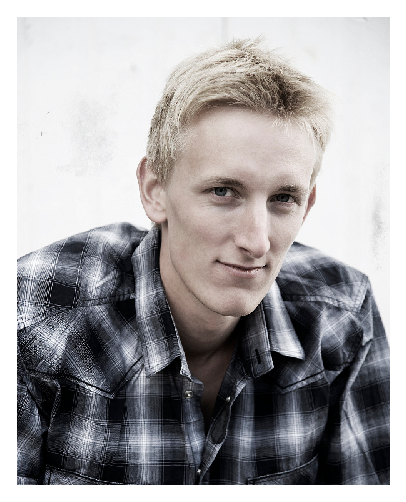
\includegraphics[width=1in,height=1.25in,clip,keepaspectratio]{bio/jo_inge.eps}}]{Jo Inge Buskenes}
received the B.Sc. degree in electrical engineering from Gj\o{}vik College University, Norway, in 2007, and the M.Sc. degree in instrumentation for particle physics from the University of Oslo, Norway, in 2010. He is currently pursuing the Ph.D. degree in image reconstruction and technology at the University of Oslo.

His industry experience includes the European Organization for Nuclear Research (CERN), Geneva, Switzerland (2007-2008), and the Norwegian Defence Research Establishment, Kjeller, Norway (2009). He has lectured in digital signal processing at the Gj\o{}vik College University (2009), and at the University of Oslo (2010-2013). His research interests include adaptive beamforming, digital image reconstruction, high performance computing, intelligent detector design and open source software.
\end{IEEEbiography}